\documentclass[11pt, letterpage, twocolumn]{article}
\usepackage{amsmath}
\usepackage{graphicx}

\begin{document}

\section{Selected Topics}
\subsection{Power Spectrum and Filtering}
To investigate the properties of the power spectrum and the effects of
filtering, we consider the simple discretely sampled sinusoidal signal:
\begin{equation}
  V_j = A \sin(2 \pi f t_j - \phi)
  \label{eq:sine}
\end{equation}

%%%%%%%%%%%%%%%%%%%%%%%%%%%%%%%%%%%%% 
% SHOW POWER IS CONFINED TO ONE BIN
%%%%%%%%%%%%%%%%%%%%%%%%%%%%%%%%%%%%%

\subsubsection{Power Spectra}
The power spectrum of a continuous signal is simply the square of the continuous
Fourier transform. However, when computing the power spectrum of a discretely
sampled signal, the leakage of power from some frequencies to others is a
problematic result of the digitization of the signal. To illustrate this, the
power spectra for two slightly different frequencies are considered: $f = 60$Hz
and $f = 59.673$Hz. These 

\begin{figure}
  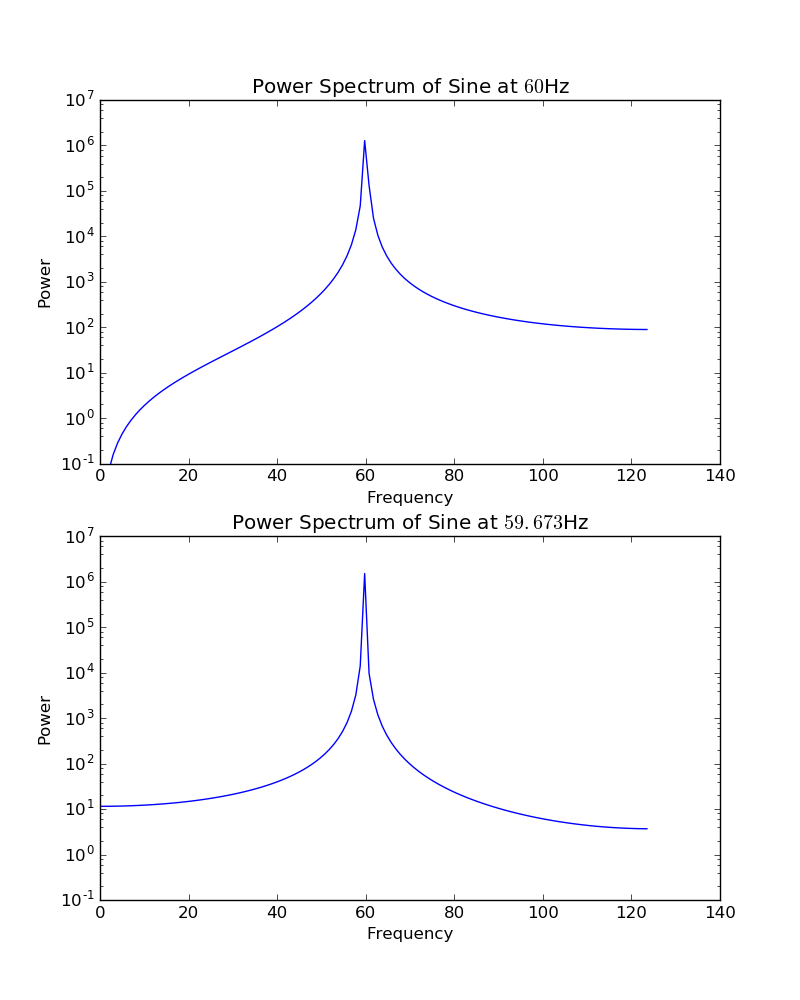
\includegraphics[width=\linewidth]{power_spectrum.png}
  \caption{
    The power spectra of equation \ref{eq:sine} with two very close
    frequencies. These signals were generated with $250$ samples with
    a sampling rate of $125$Hz.
  }
  \label{}
\end{figure}

\subsubsection{Windows}
One of the standard ways to reduce spectral leakage is to multiply the data in
time space with a window before performing the Fourier transform. The
window should be equal to zero outside of the desired interval, thus
creating a window where the signal exists. All discretely sampled
signals can be thought of as having a rectangular window from when
sampling began to the most recent measurement. Two of the
most common windows we look into are the Hann window and the Blackman-Harris
window. The Hann function and its Fourier transform are shown in figure
\ref{fig:hann_window}. In time space, it is akin to applying part of a
cosine wave to the signal. In frequency space, however, it can be
interpreted as applying a convolution to Fourier transform of the
signal. 

\begin{figure}
  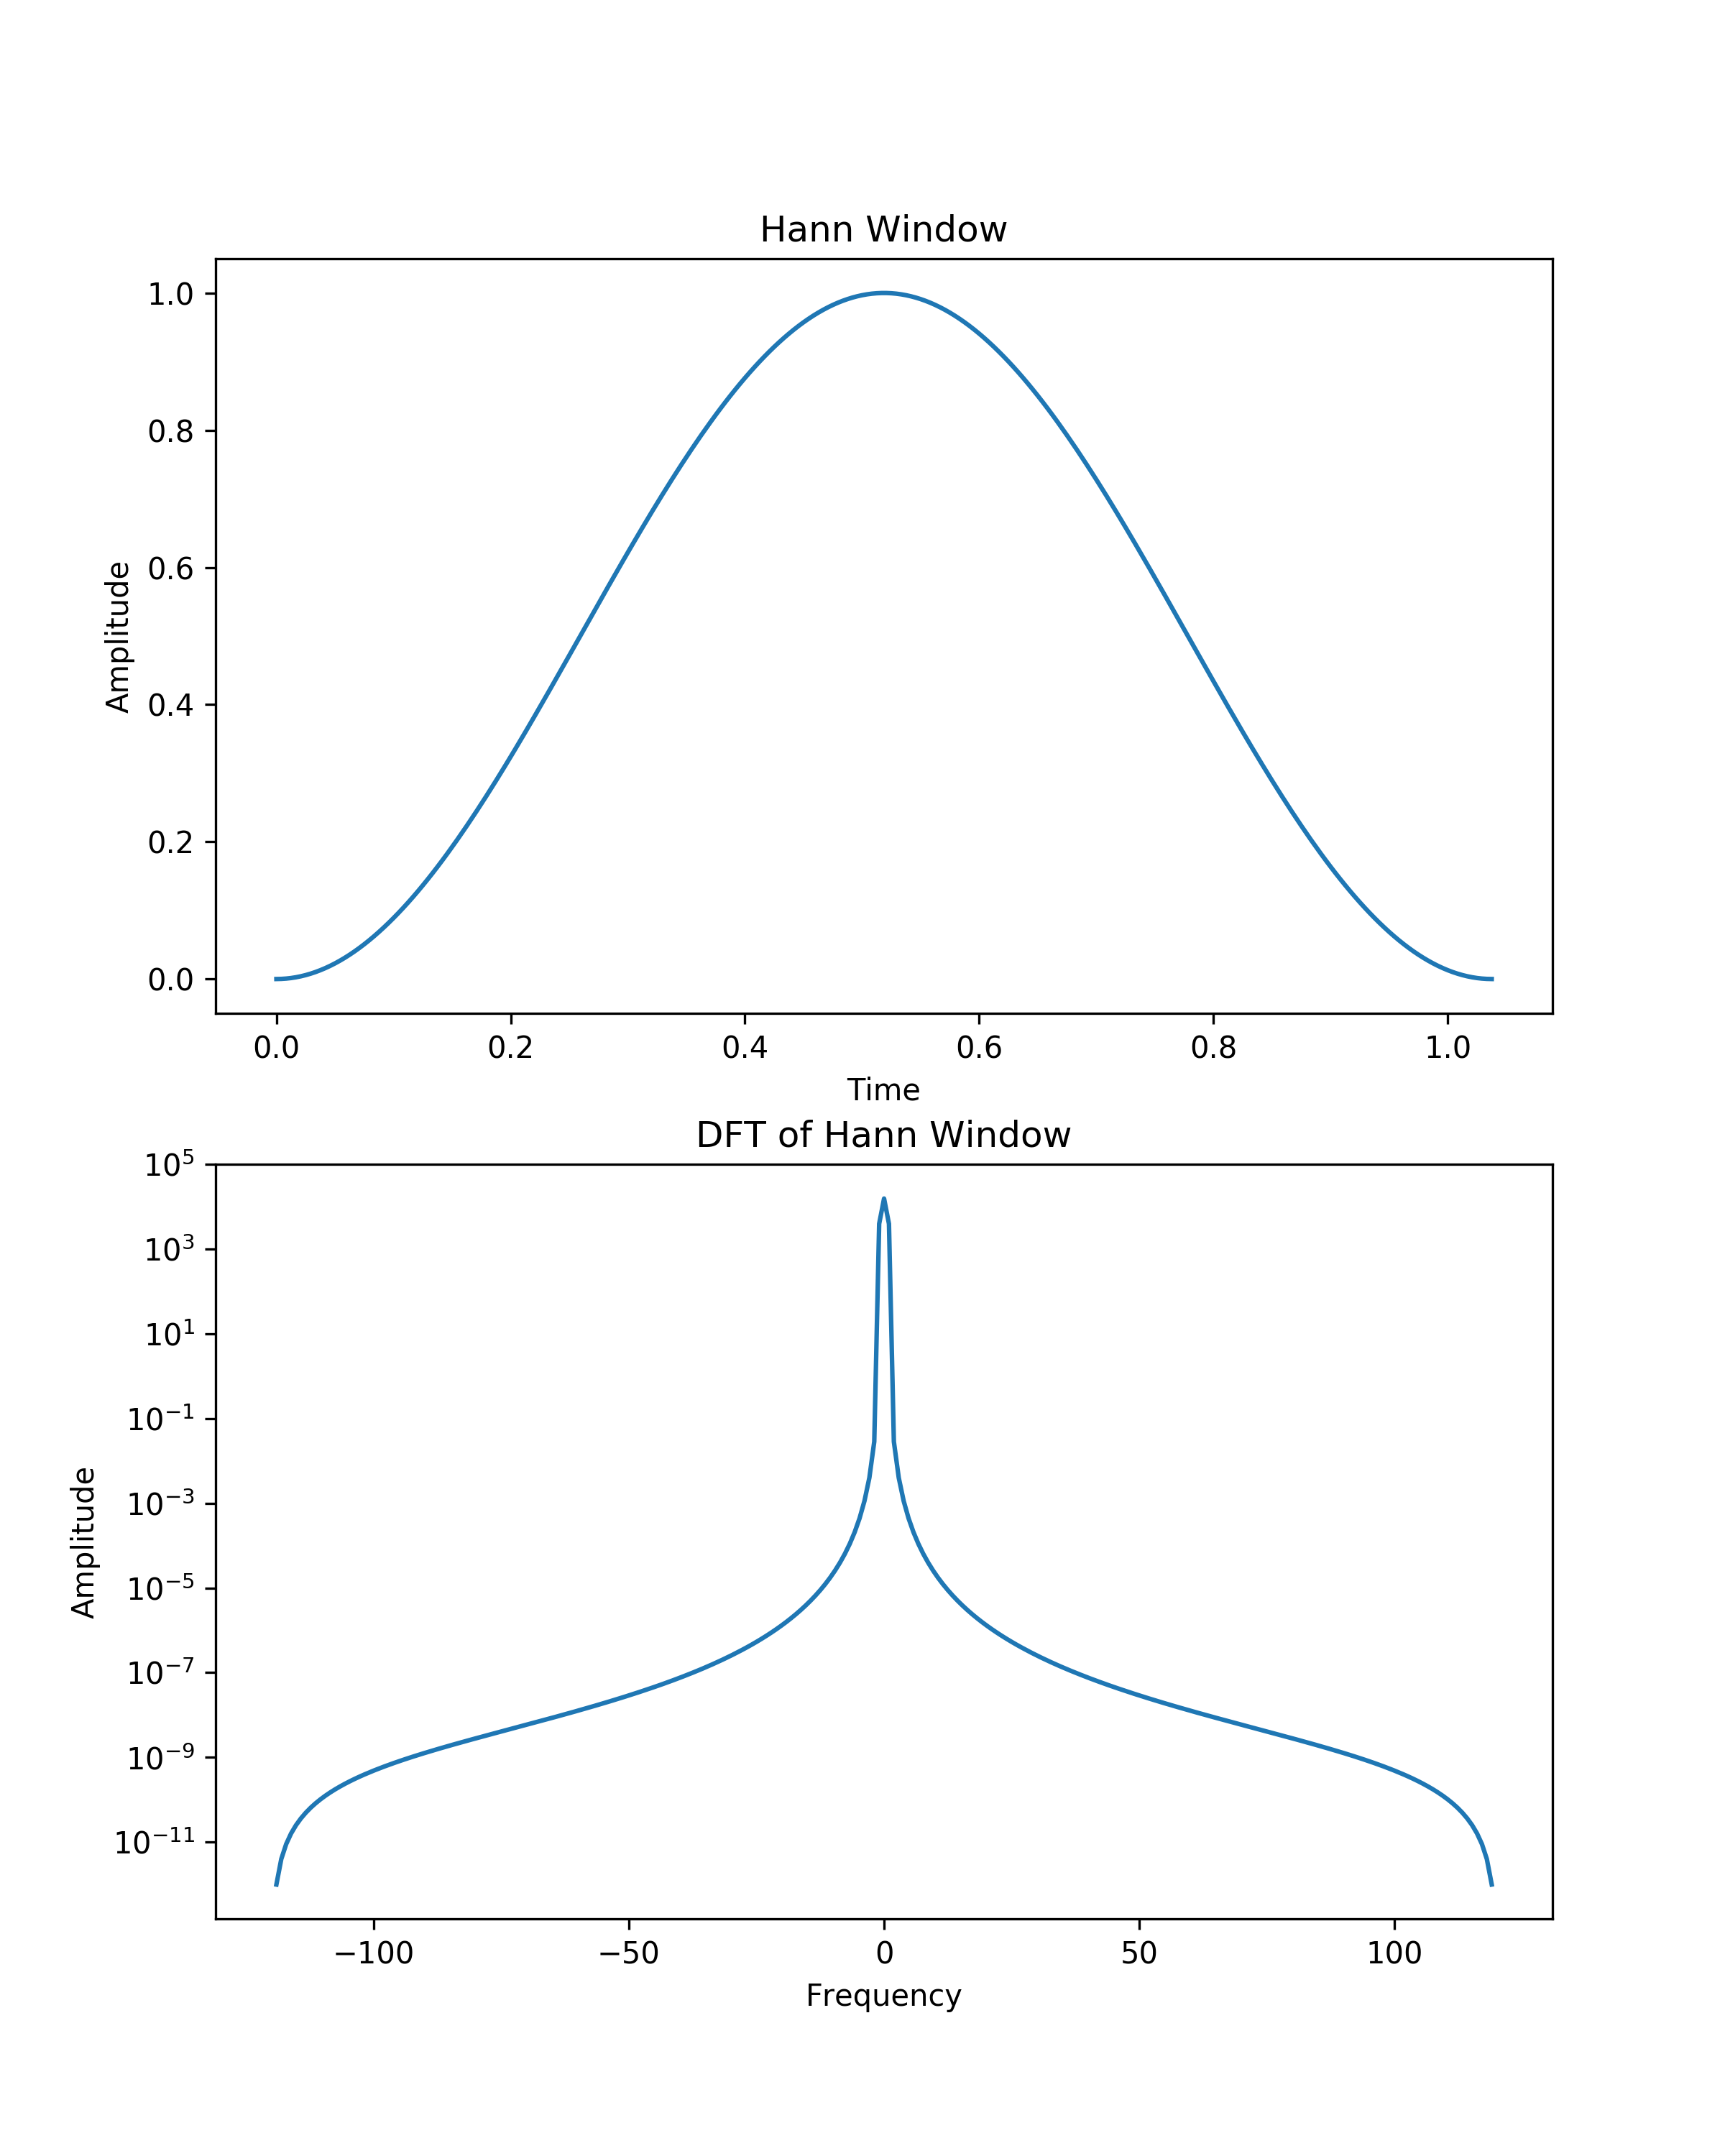
\includegraphics[width=\linewidth]{hann_window.png}
  \caption{
    The Hann window (top) and its Fourier transform (bottom). It can be thought
    of as a portion of a cosine wave.
  }
  \label{fig:hann_window}
\end{figure}

Now the Hann window can be applied to the two signals that were used previously
with frequencies $60$Hz and $59.673$Hz, shown in figures \ref{fig:hann_0} and
\ref{fig:hann_1}, respectively. The windowed function, shown in the
top panel of figure \ref{fig:hann_0}, now has an envelope, but there are also smaller beats that
appear to emerge which are not actually in the signal. This is
reflected in the power spectrum, shown in the lower panel, where the
peak has broadened the peak but has also decreased the power for the
higher frequencies. These similar effects can also be seen in figure
\ref{fig:hann_1} for the frequency $f = 59.673$, though the
higher frequencies reduced even further.

\begin{figure}
  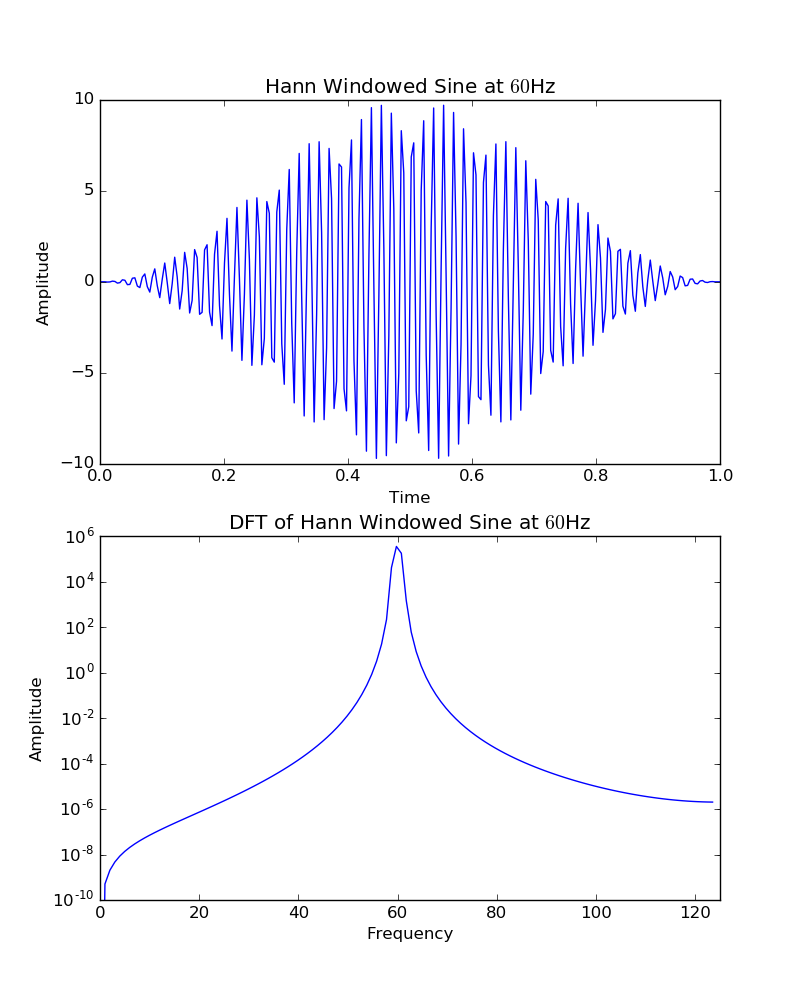
\includegraphics[width=\linewidth]{hann_0.png}
  \caption{
    The Hann window applied to equation \ref{eq:sine} with $f = 60$Hz in time
    space (top) and in frequency space (bottom).
  }
  \label{fig:hann_0}
\end{figure}

\begin{figure}
  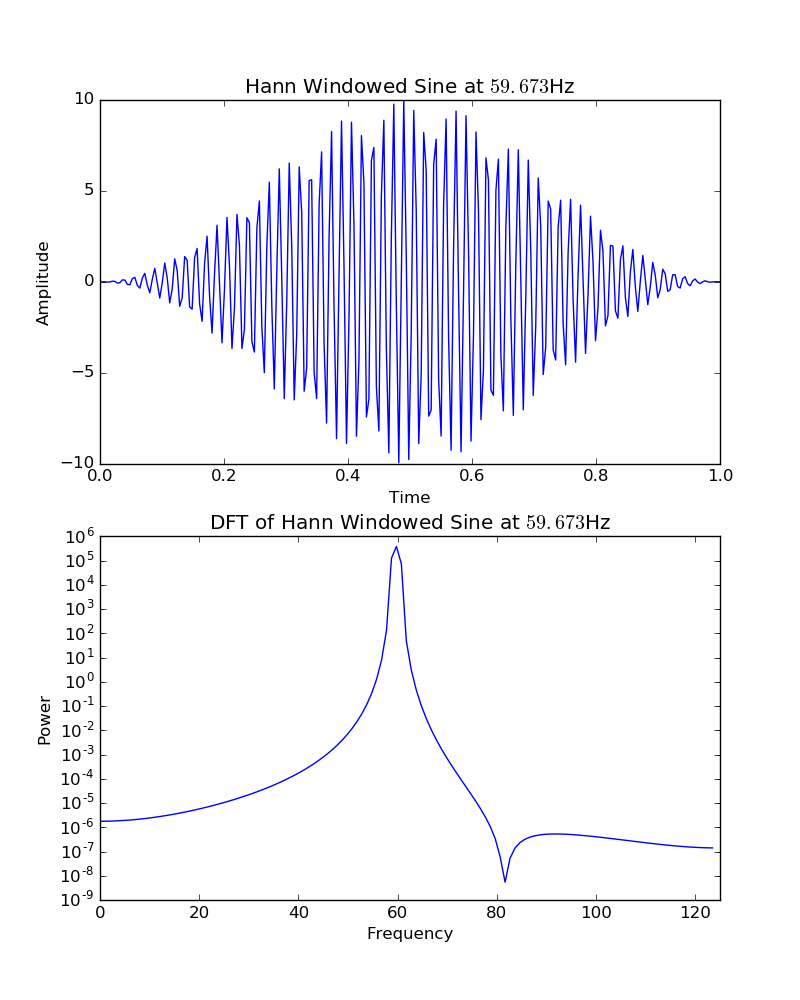
\includegraphics[width=\linewidth]{hann_1.png}
  \caption{
    The Hann window applied to equation \ref{eq:sine} with $f = 59.673$Hz in
    time space (top) and in frequency space (bottom).
  }
  \label{fig:hann_1}
\end{figure}

We can compare the results of using the Hann window with the
Blackman-Harris window, shown in figure \ref{fig:blackman_harris}. The Fourier transform of the Blackman-Harris
window has a very distinct local minima around the peak. When this is
applied to the signal, the peaks at $60$Hz also have distinct minima
around them. However, this also widens the peak and decreases the
power of the surrounding frequencies.

\begin{figure*}
  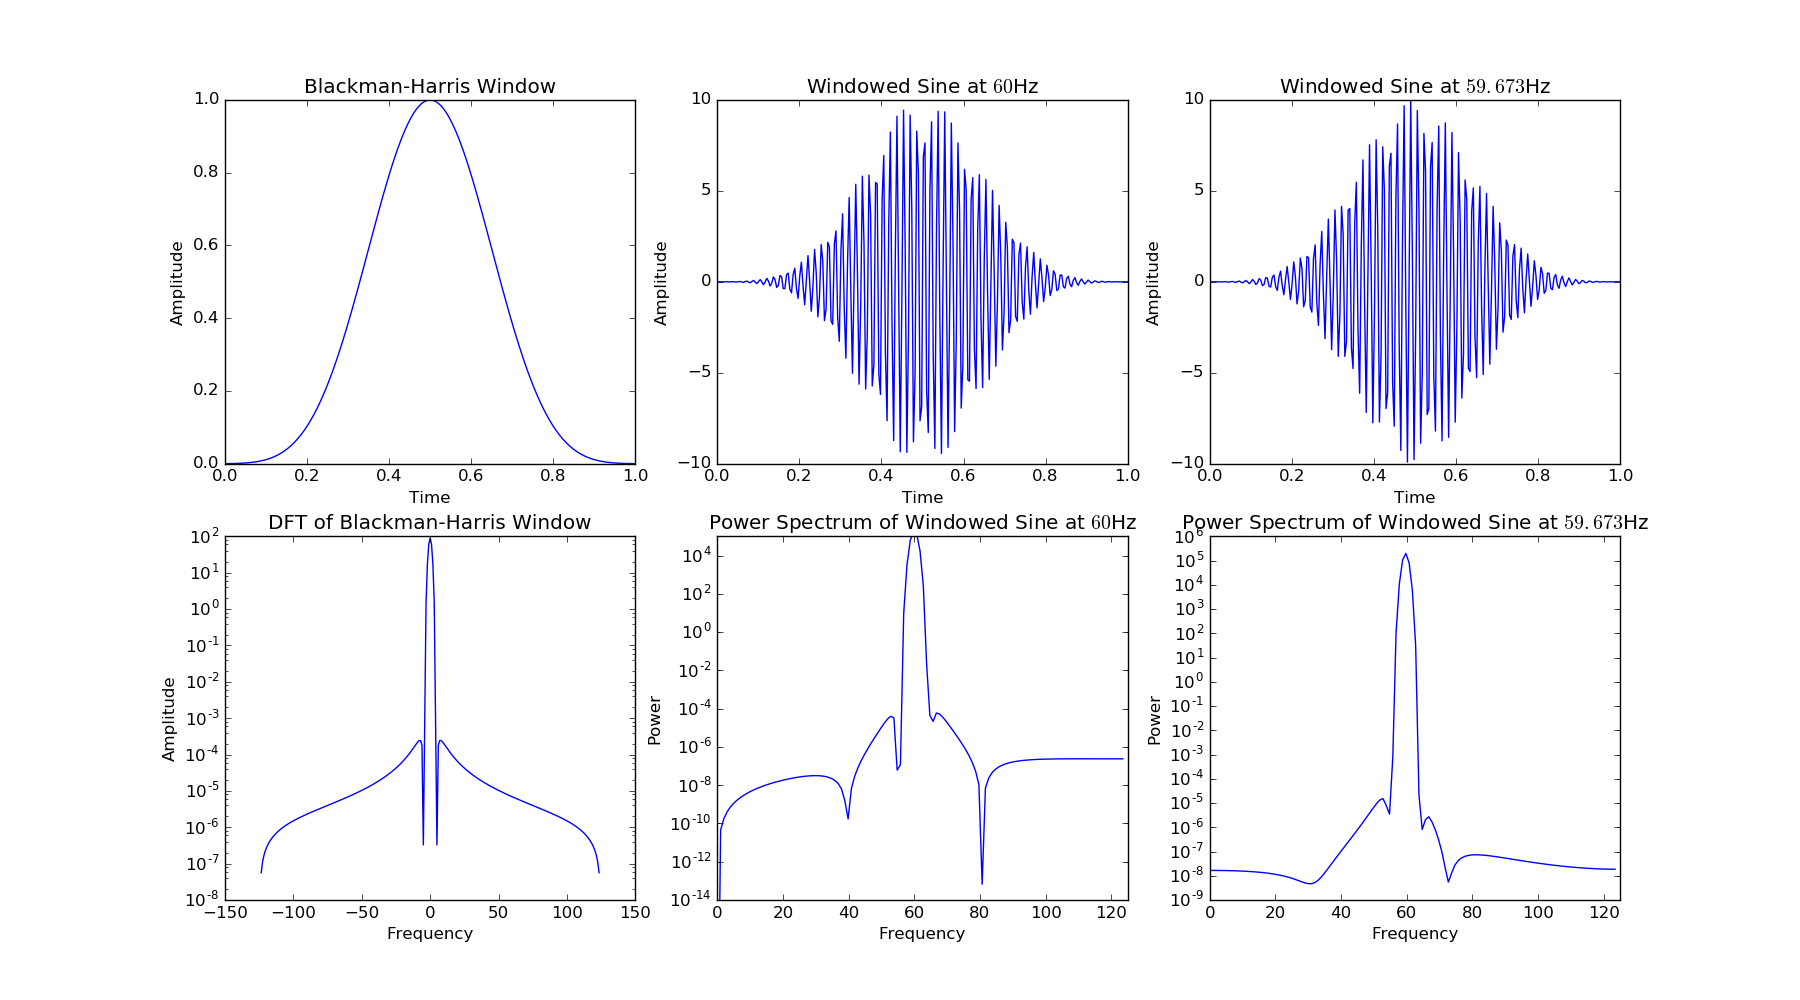
\includegraphics[width=\linewidth]{blackman_harris.png}
  \caption{
    The Blackman-Harris window is also applied to equation \ref{eq:sin} with
    frequencies $f = 60$Hz and $f = 69.673$Hz. The functions in time space are
    shown in the top row while the bottom row shows the Fourier transform of the
    Blackman-Harris window and the power spectra of the functions above.
  }
  \label{fig:blackman_harris}
\end{figure*}

\section{General Applications}

\subsection{Heart Beats}
The data gives a time sequence of heart beats sampled at $125$Hz. Since the data
is evenly sampled and the number of samples is a power of two, padding is not
necessary in this case. The amplitude spectrum is shown in figure
\ref{fig:beats}. The two most dominant frequencies are approximately $2$Hz and
$4$kHz, with corresponding periods $0.5$s and $0.25$s, respectively.

\begin{figure}
  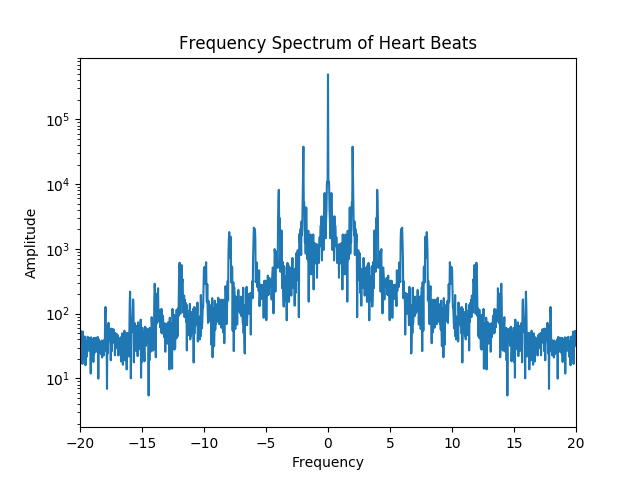
\includegraphics[width=\linewidth]{beats.png}
  \caption{
    The amplitude spectrum of the patient's heart beats. The data was sampled at
    $125$Hz and has $4096$ samples.
  }
  \label{fig:beats}
\end{figure}

The average resting heart rate is about $60$ to $100$ beats per minute. However,
this translates to periods within a range of $1$s to $1.6$s, which are
significantly faster than that of the patient. This would suggest that the
patient was not at rest before the measurement or some other reason for a faster
heart rate. The $2$Hz heart rate can be explained through the patient
exercising or a medical condition. However, the heart rate of $4$Hz,
or $240$ beats per minute, is much more unrealistic. There are peaks
that occur periodically as the frequency axis increases, and may be an
artifact of sampling.

\subsection{Financial Series}
For this section, we analyze the stock prices for 6 companies, shown in figure
\ref{fig:stocks_time}.

\begin{figure}
  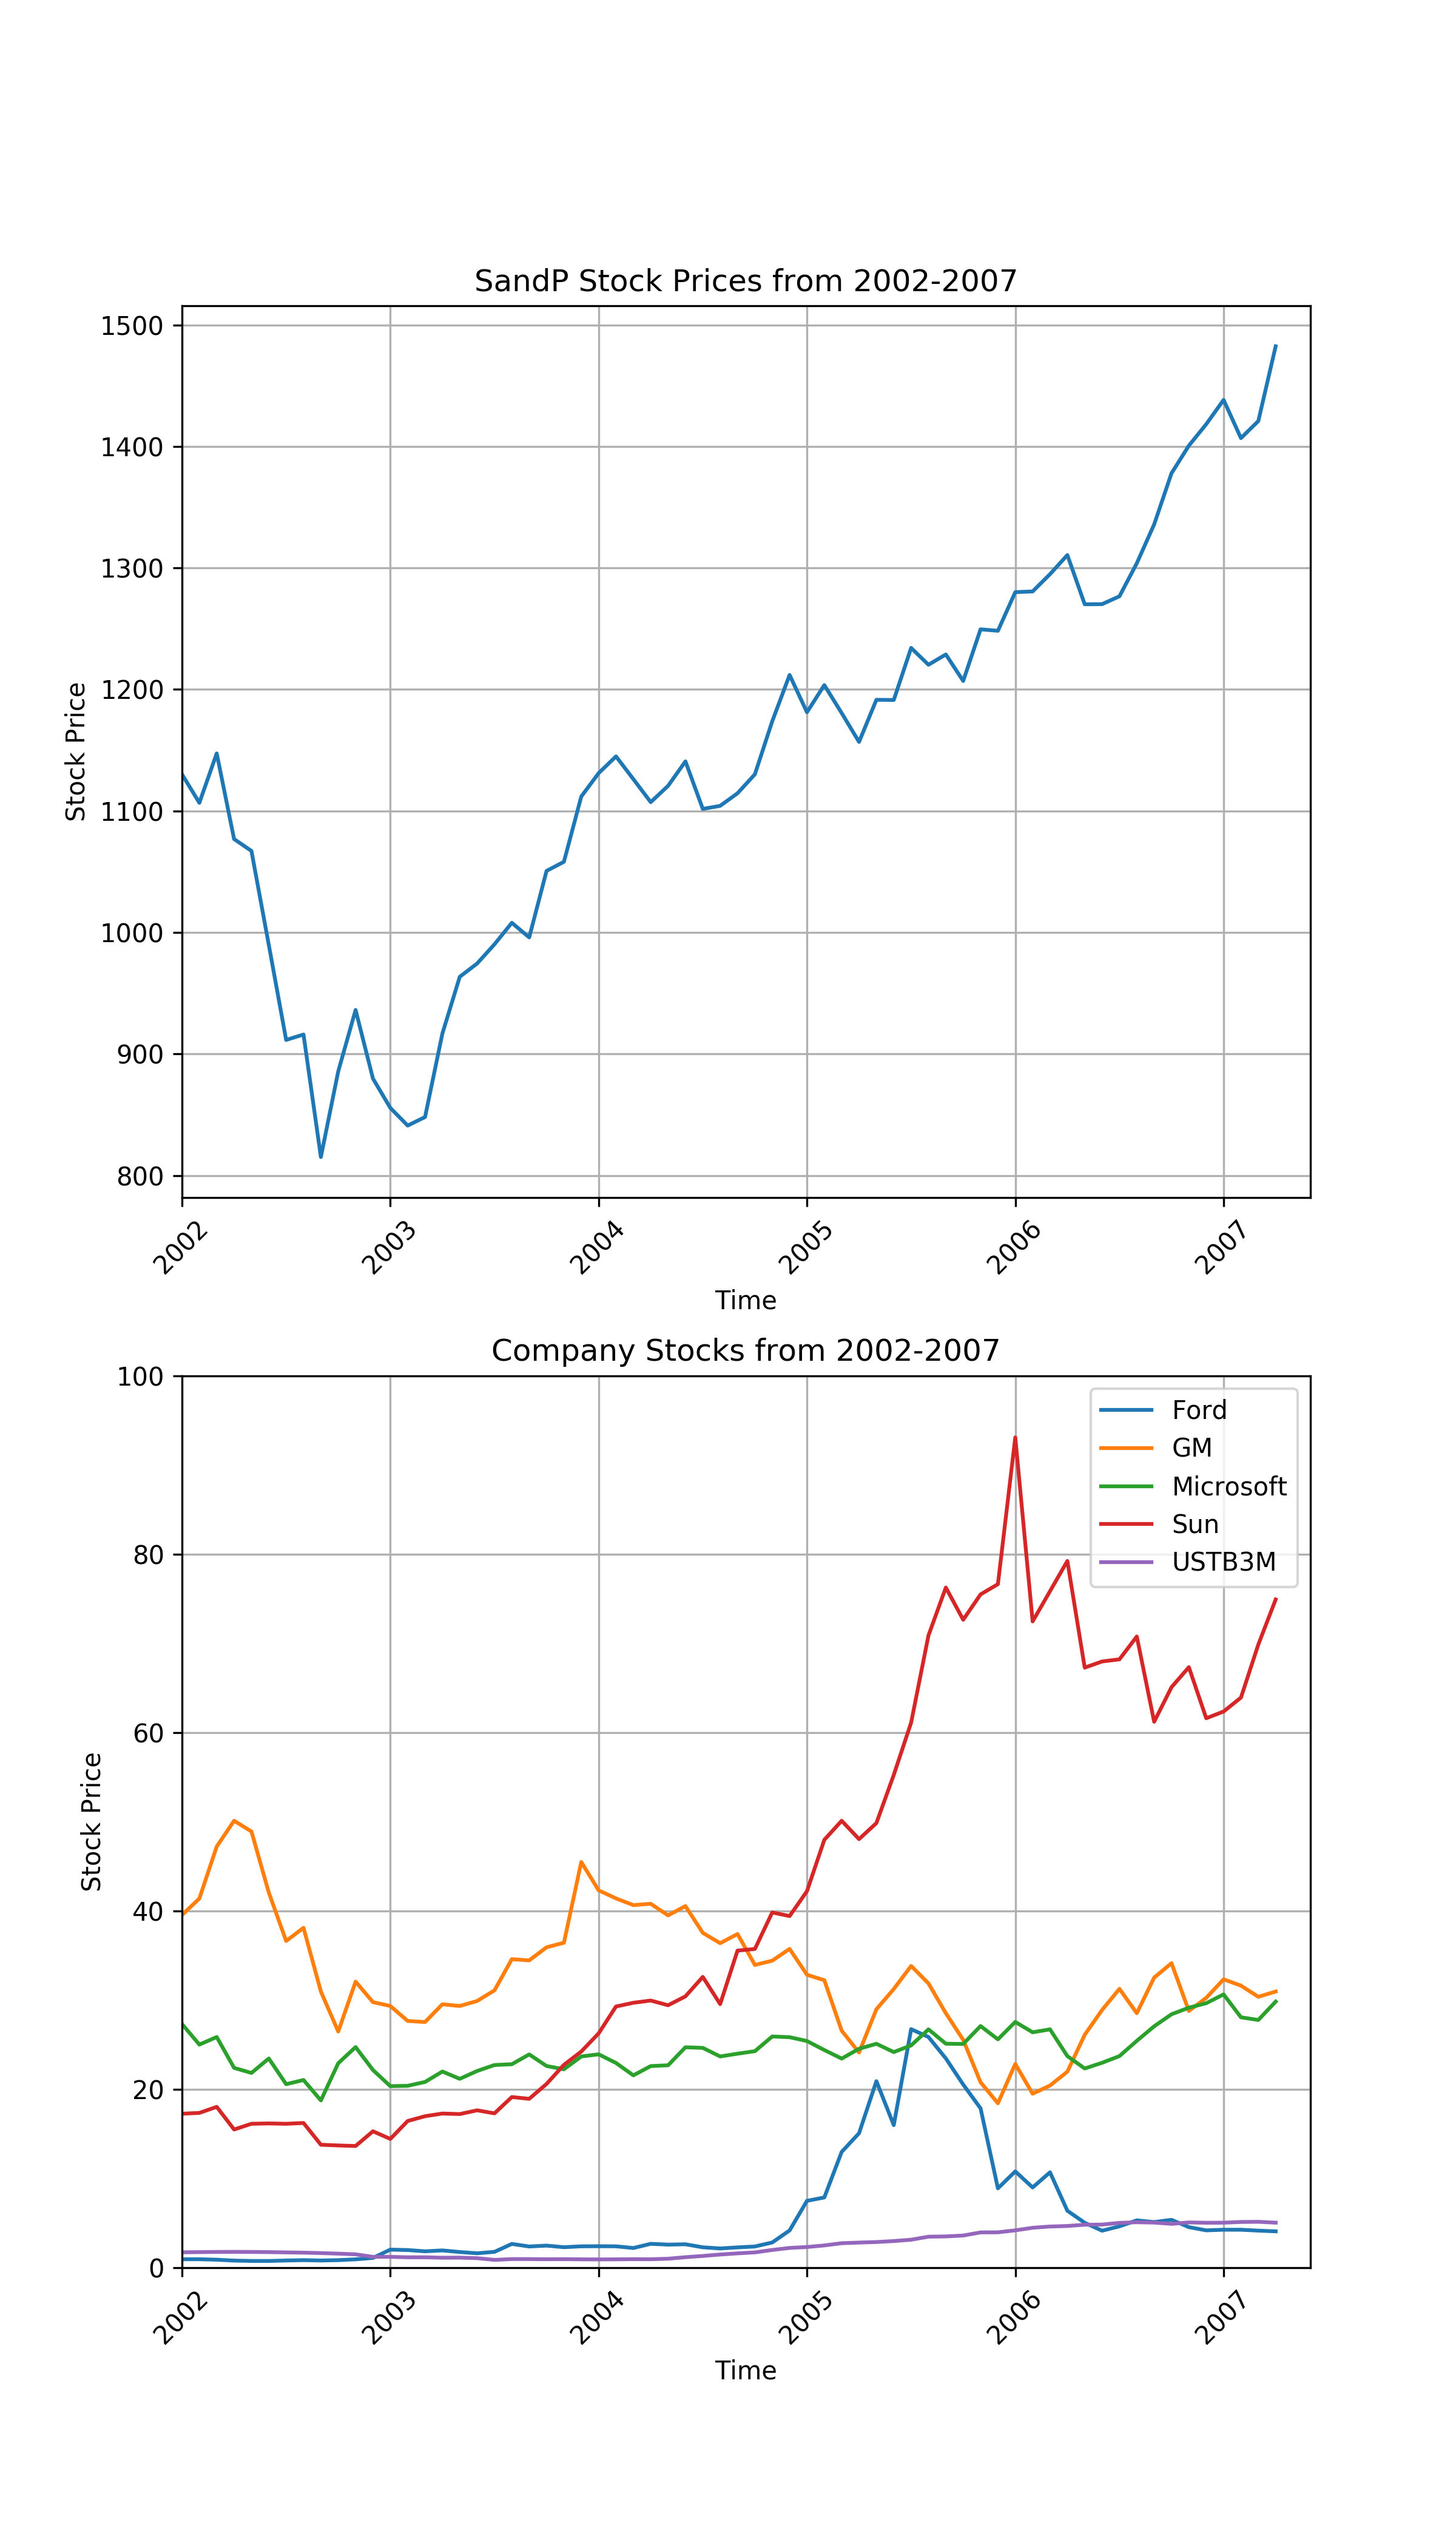
\includegraphics[width=\linewidth]{stocks_time.png}
  \caption{
    The monthly stock prices of six companies from $2002$ through to mid-$2007$.
  }
  \label{fig:stocks_time}
\end{figure}

This data is then used to compute the continuously compounded returns $R_i$,
given by the relation:
\begin{equation}
  R_i = \ln\left( \frac{P_i}{P_{i-1}} \right)
  \label{ccr}
\end{equation}
which are shown in figure \ref{fig:stocks_returns}. The autocorrelation of the
data points are shown in \ref{fig:stocks_ac}.

\begin{figure*}
  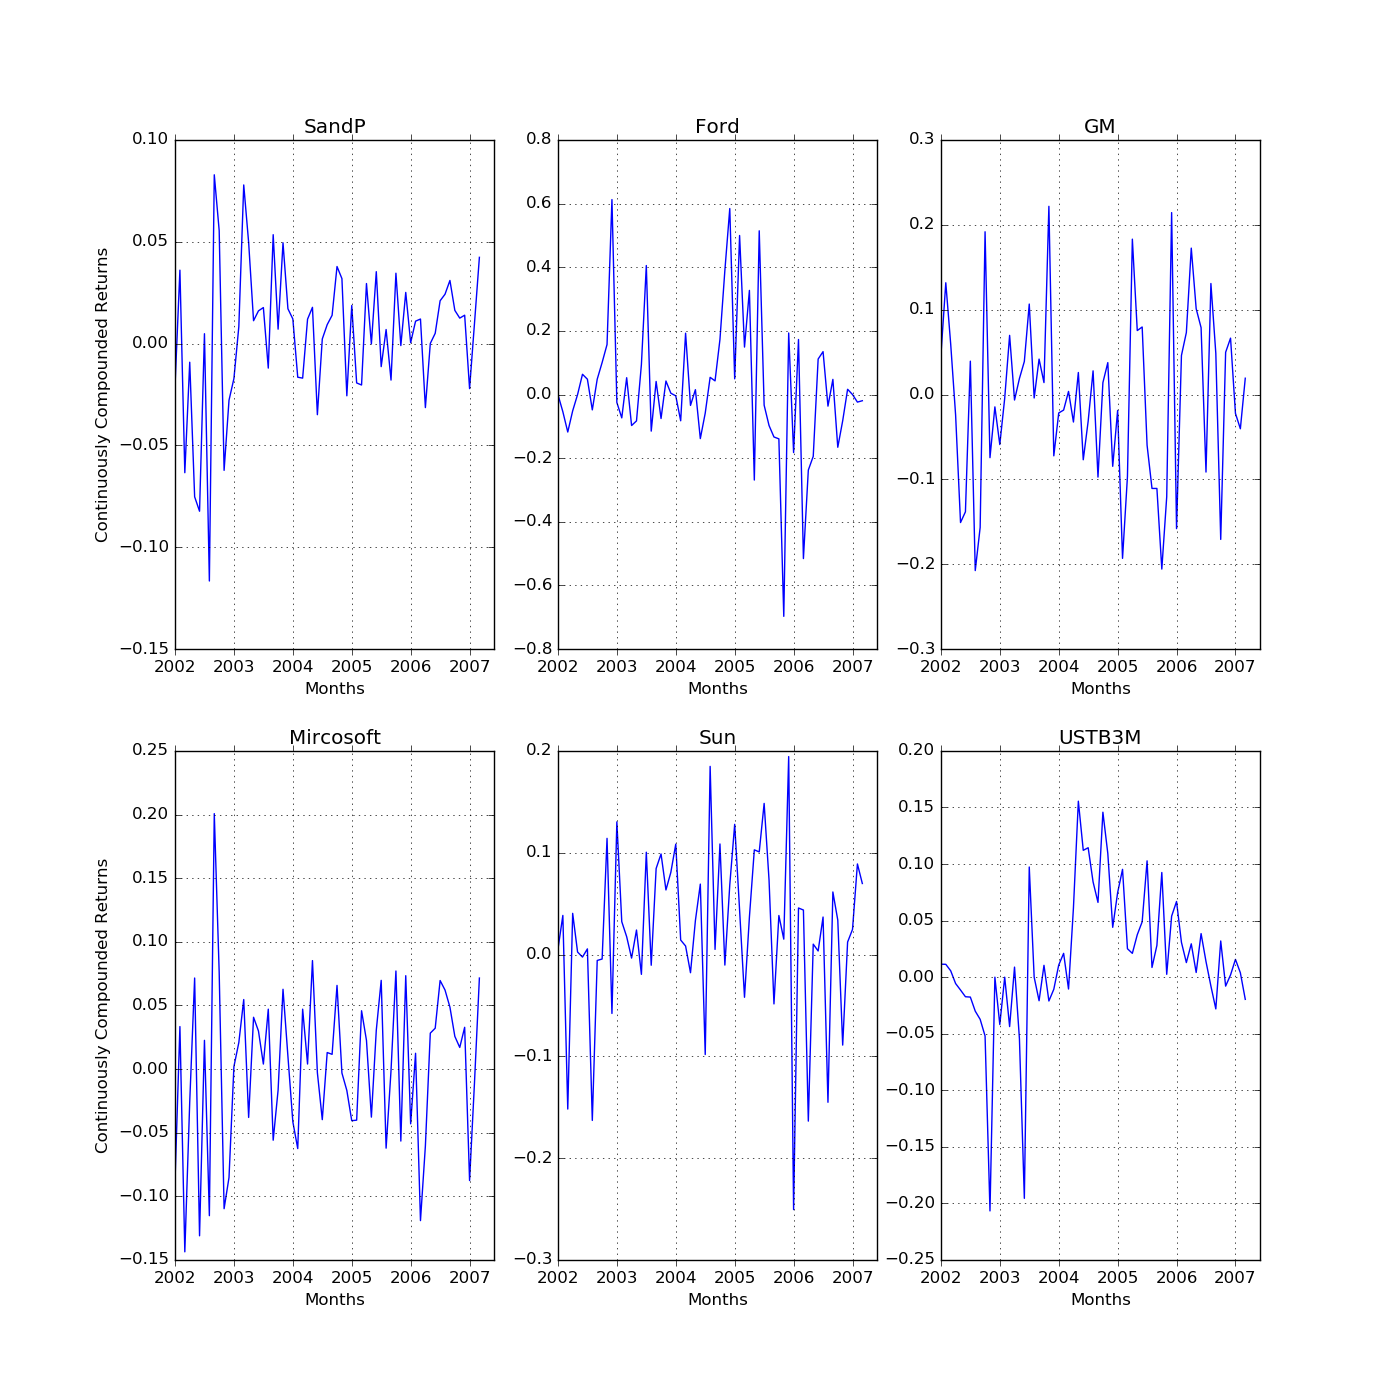
\includegraphics[width=\linewidth]{stocks_returns.png}
  \caption{
    The continuously compunded returns of six companies. The returns were
    computed from the data in figure \ref{fig:stocks_time} using equation
    \ref{ccr}.
  }
  \label{fig:stocks_returns}
\end{figure*}

\begin{figure*}
  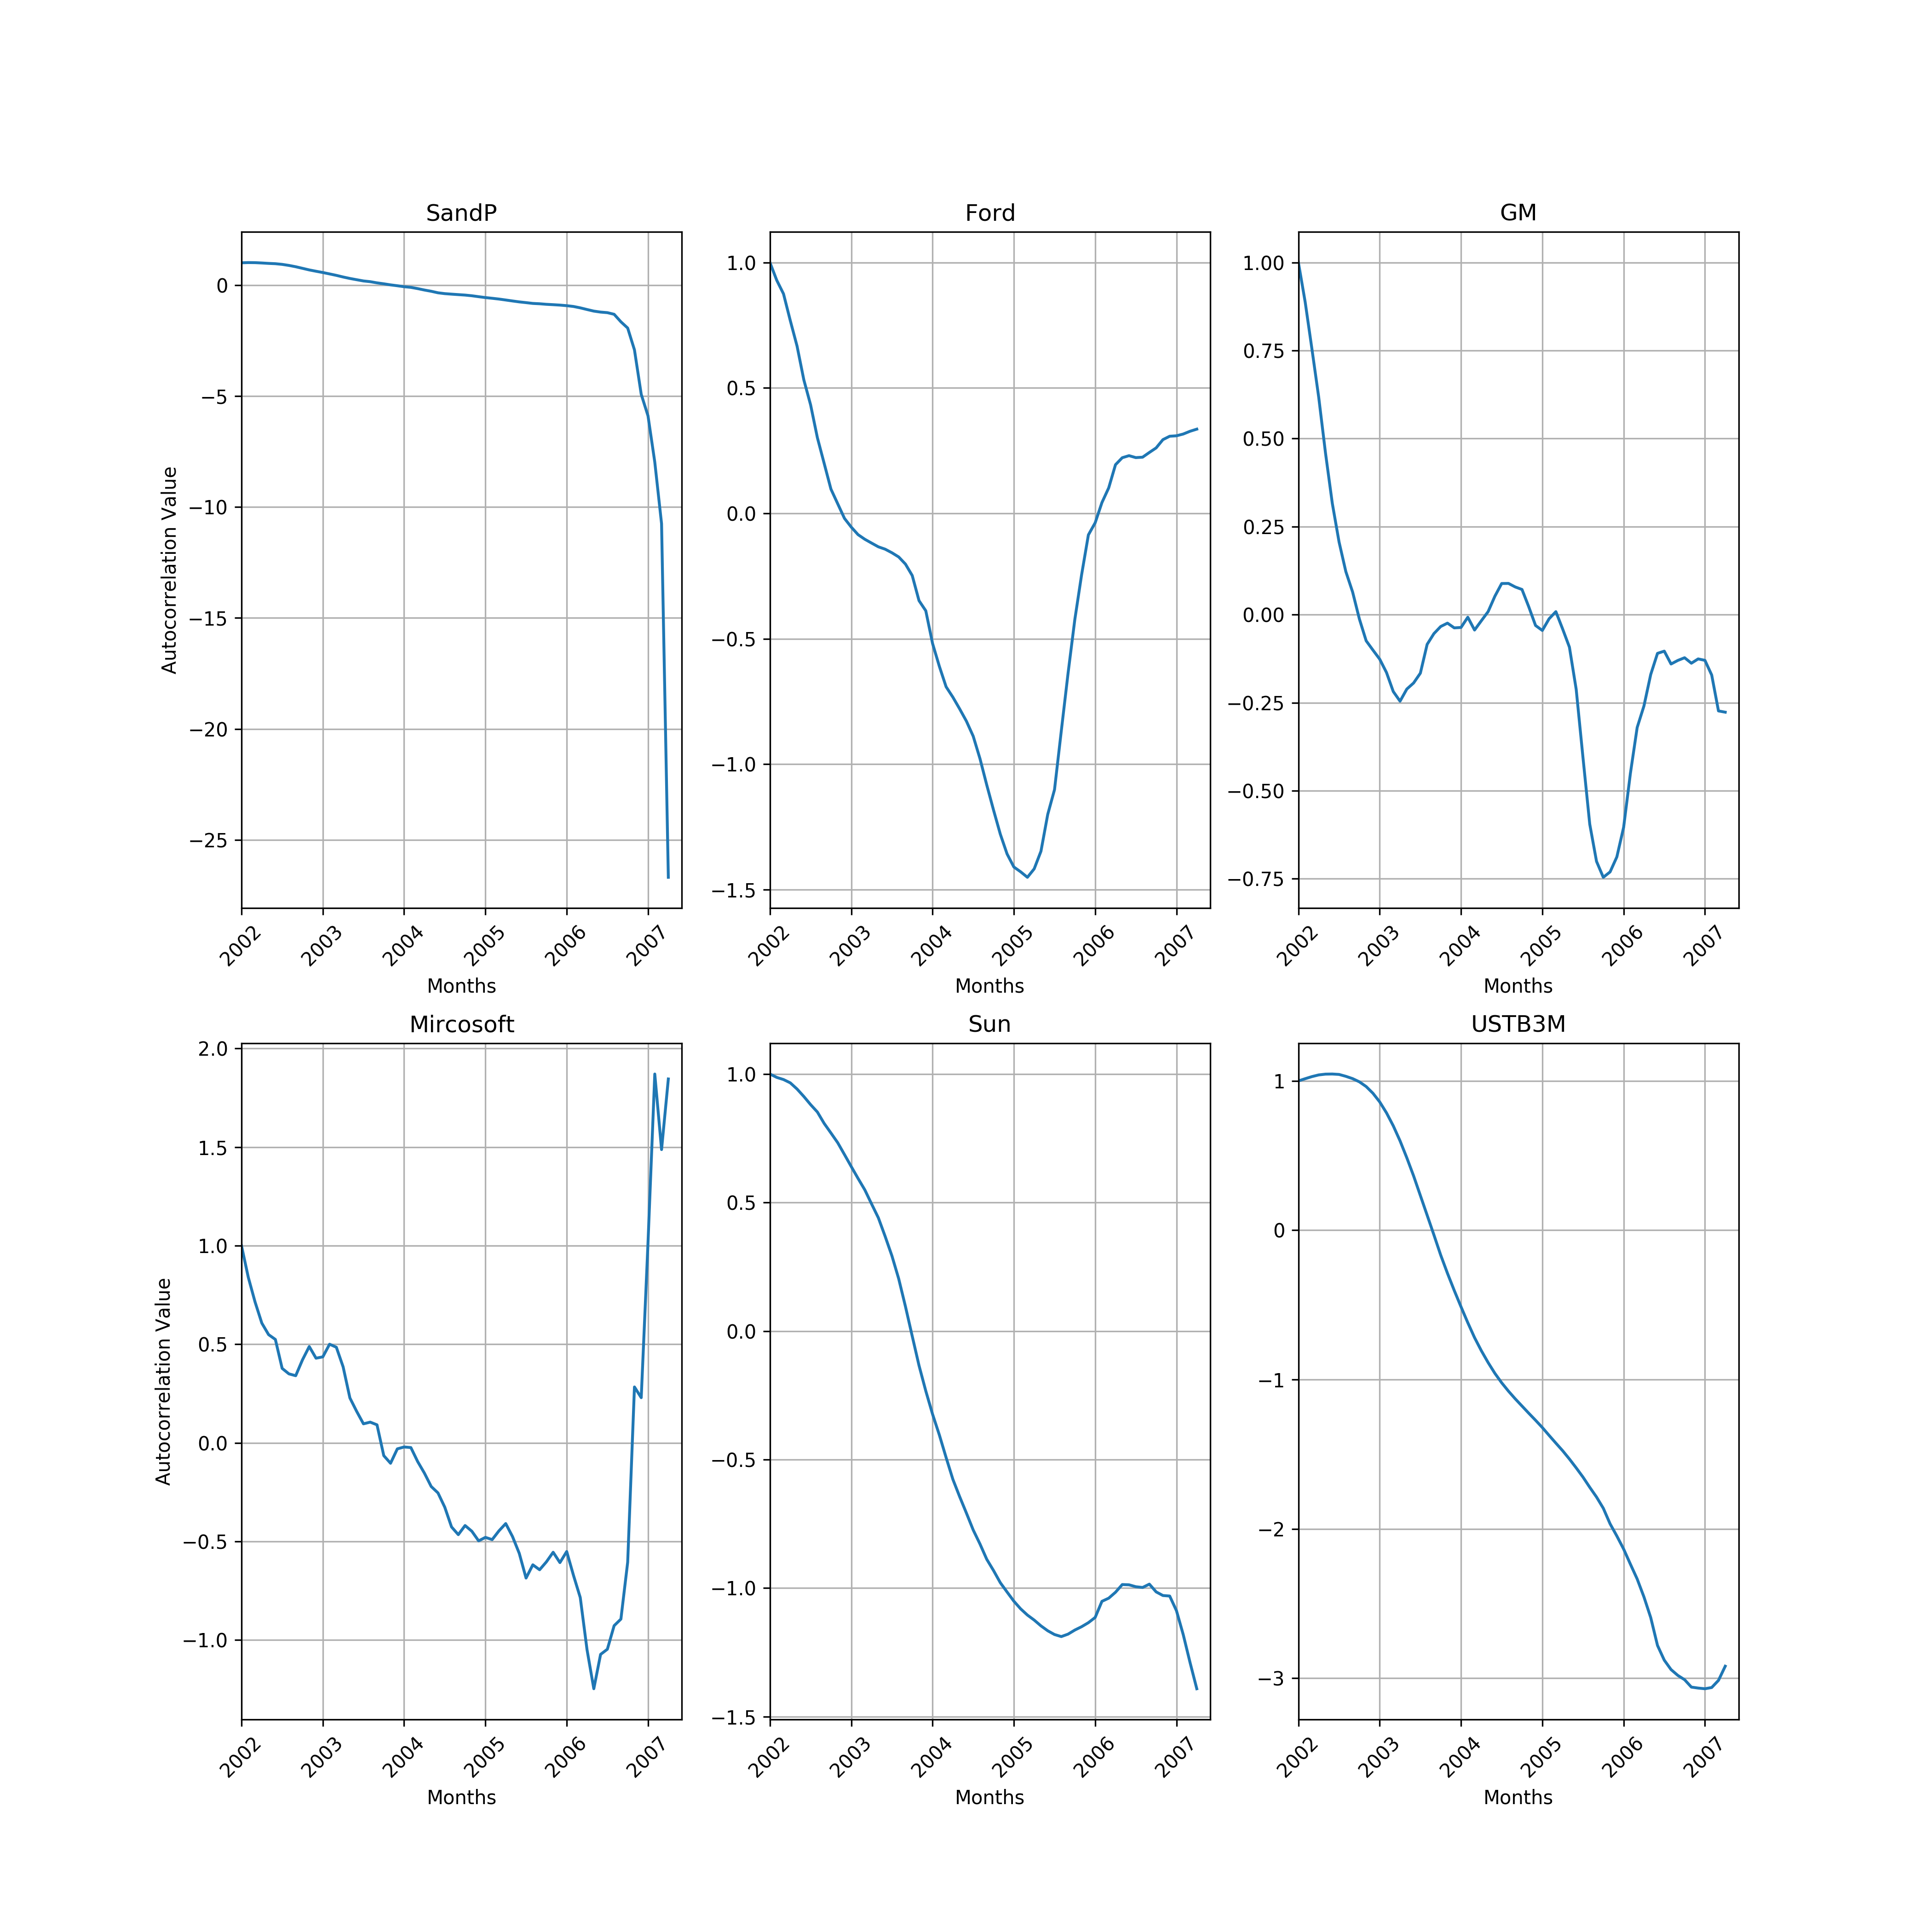
\includegraphics[width=\linewidth]{stocks_ac.png}
  \caption{
    The autocorrelation data of six companies.
  }
  \label{fig:stocks_ac}
\end{figure*}

\begin{figure*}
  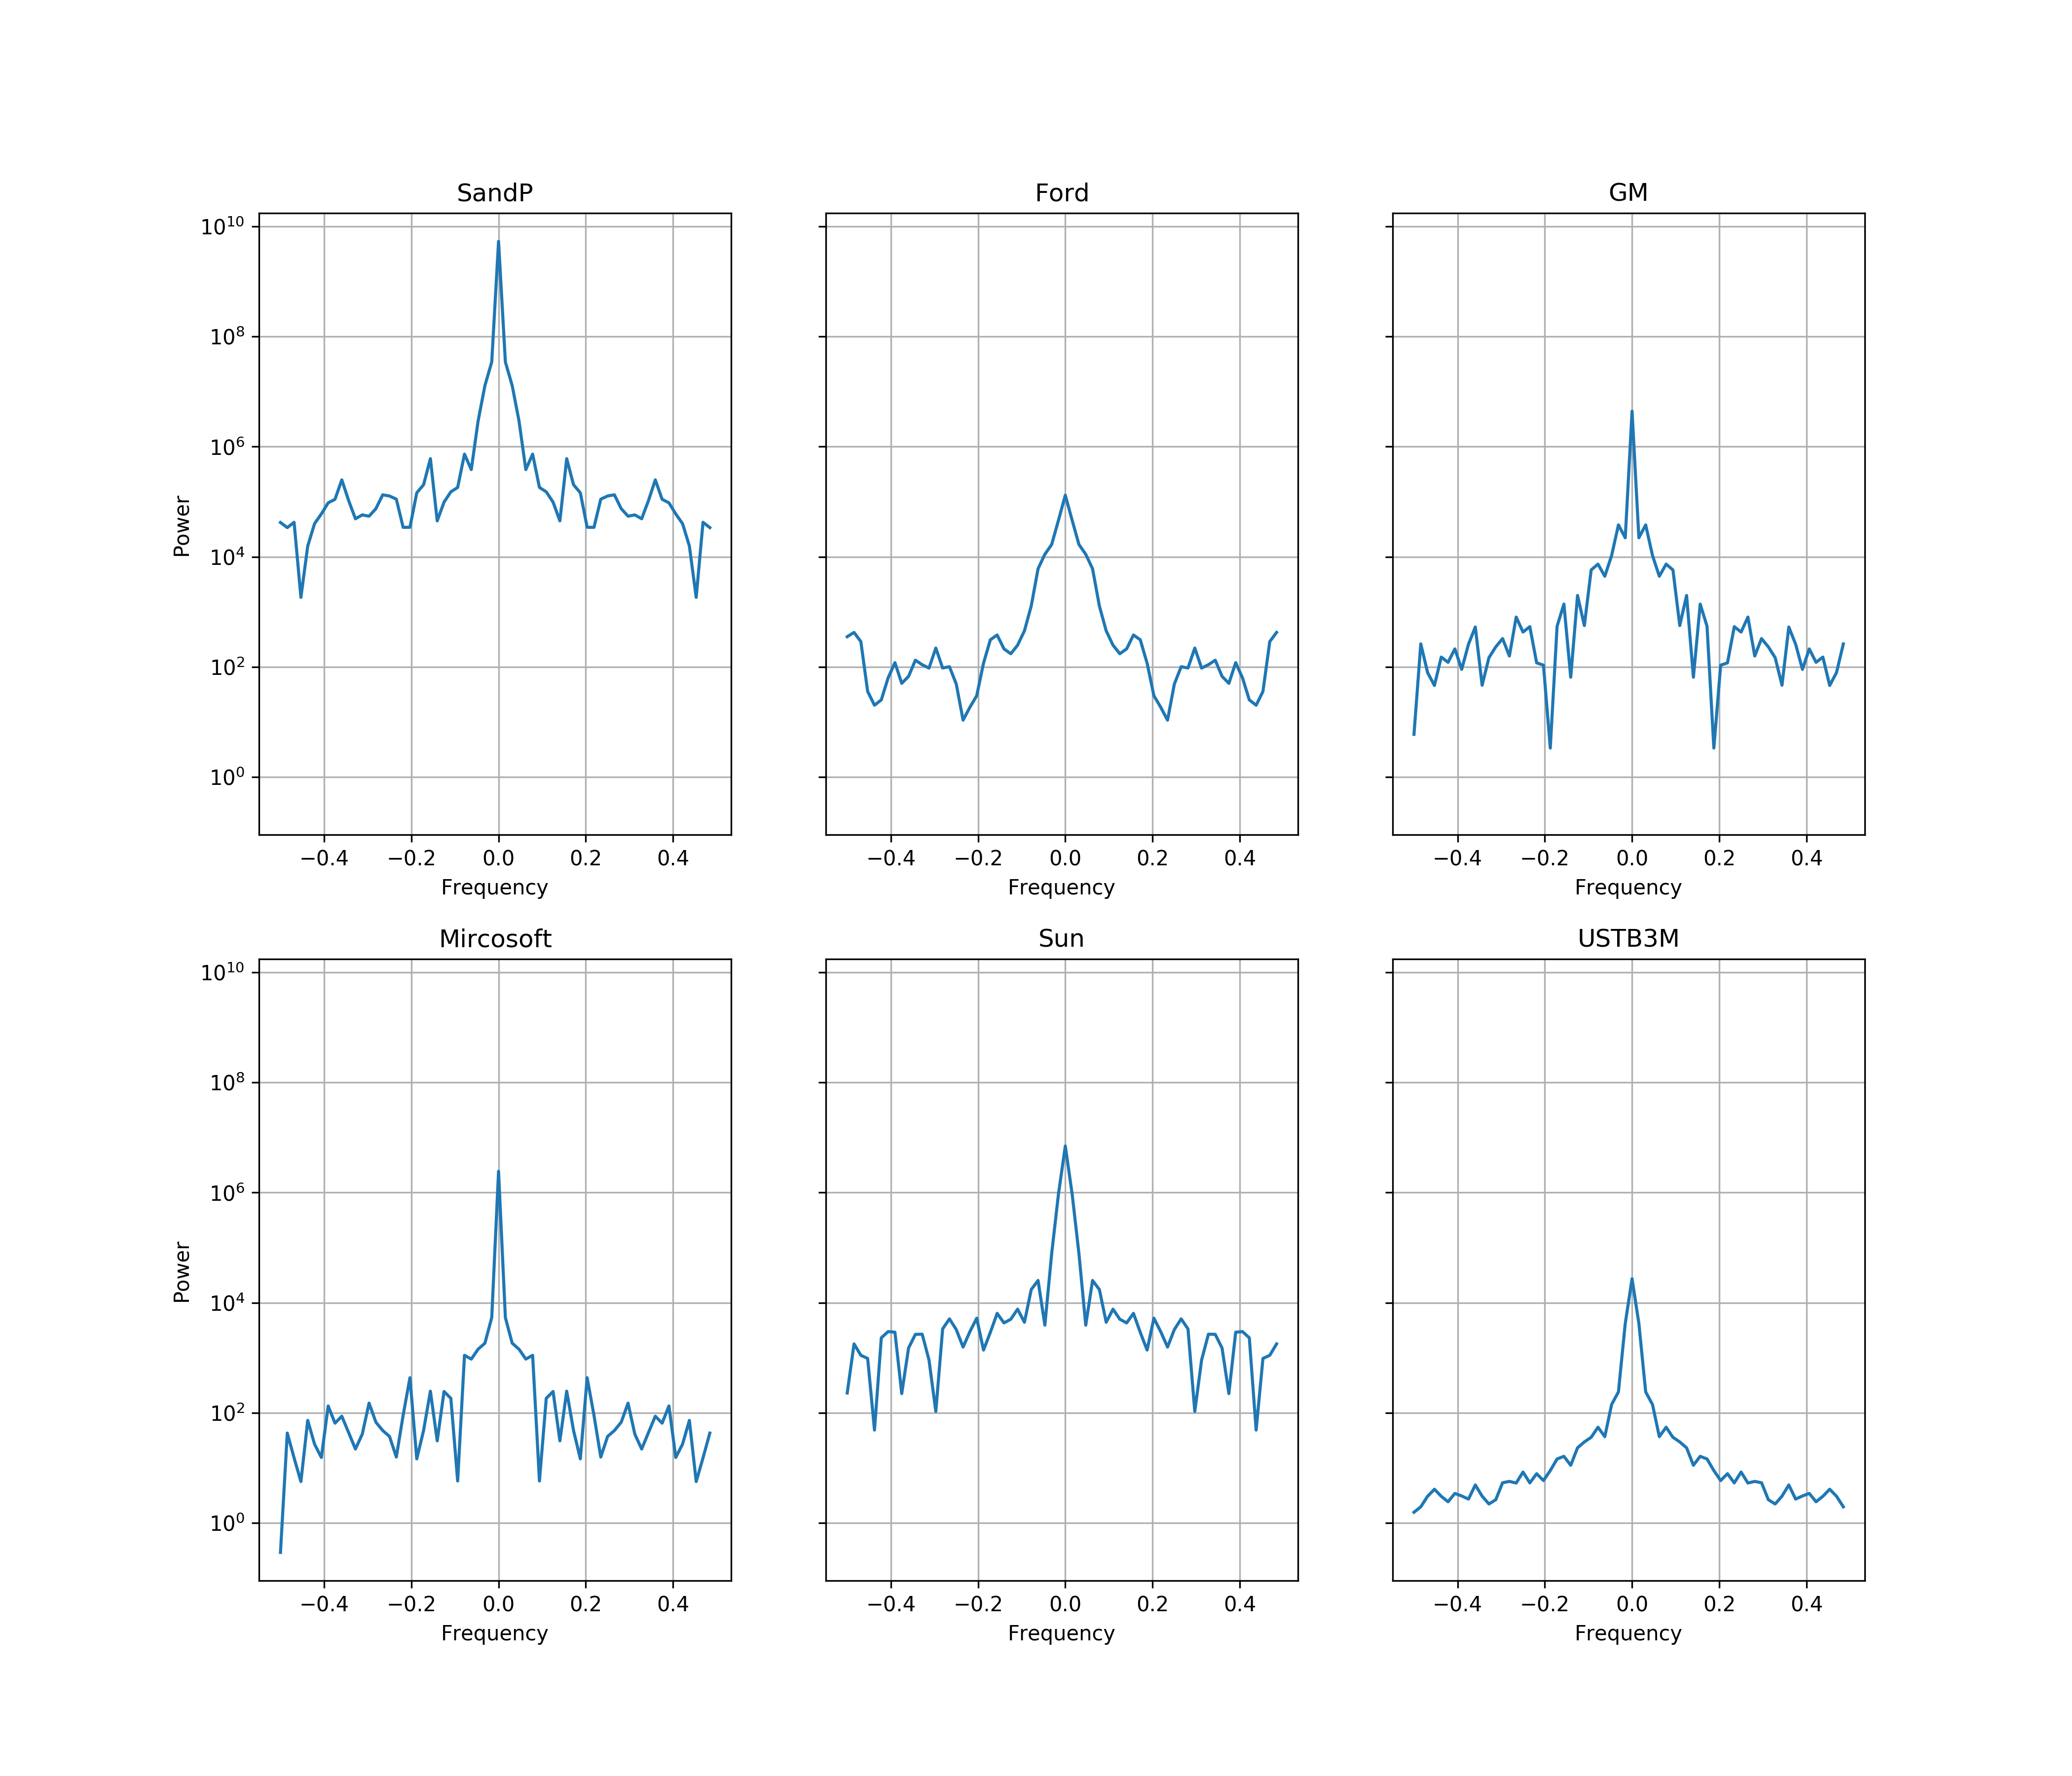
\includegraphics[width=\linewidth]{stocks_power_spectrum.png}
  \caption{
    The power spectra of the stock prices of six companies. The frequencies are
    in units of per month.
  }
  \label{fig:stocks_ps}
\end{figure*}

Next, we take a look at the daily closing value of the Dow Jones Industrial Average, which is a measure of the average stock price in the US market. In figure \ref{fig:dow}, the original data and its amplitude spectrum are shown.

\begin{figure*}
  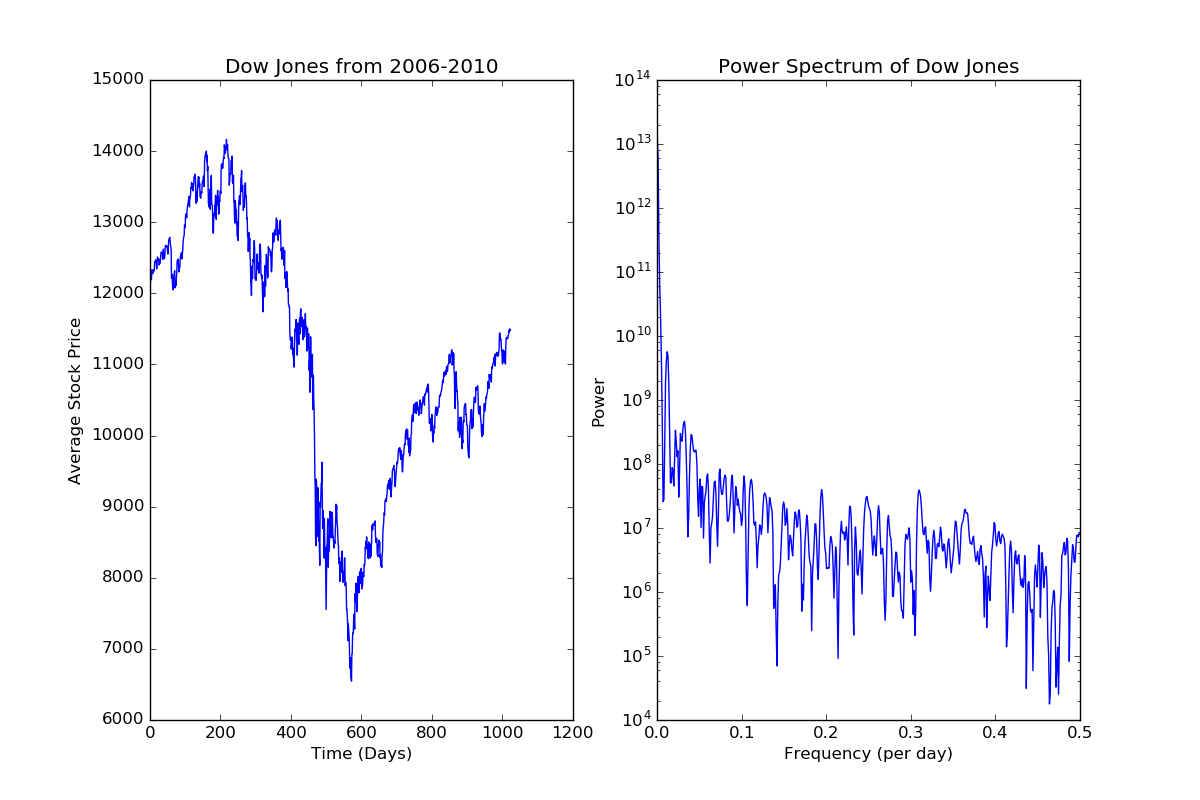
\includegraphics[width=\linewidth]{dow.png}
  \caption{
    The given data of daily average stock prices from $2006$ to $2010$ is plotted on the left and its power spectrum is given on the right.
  }
  \label{fig:dow}
\end{figure*}

\begin{figure}
  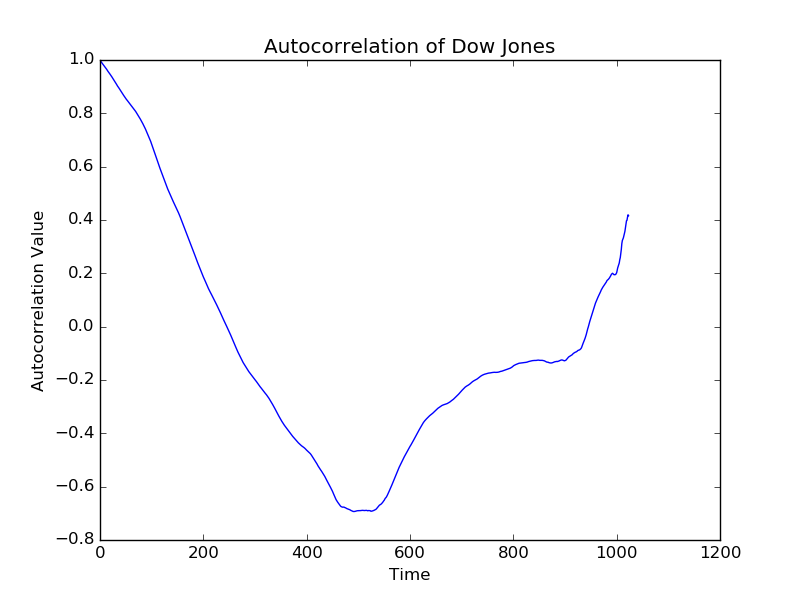
\includegraphics[width=\linewidth]{dow_ac.png}
  \caption{
    The autocorrelation values of the data shown in figure \ref{fig:dow}.
  }
  \label{fig:dow_ac}
\end{figure}

\end{document}